\section{Video QoE Parameters in YouTube and DASH-IF: A Comparison}
\label{sec:open-dash}
%\noteng{This section is weak}

This section gives a baseline comparison technique between YouTube and other DASH based protocols based on our findings on YouTube behavior for joint video quality and streaming rate adaptation. For this comparison, we consider the \ac{DASH-IF} implementation (\texttt{dash.js}) that uses a naive approach for DASHify-ing videos and adaptive video streaming based on channel quality feedback. The reference \ac{DASH-IF} implementation uses a methodology where the \ac{DASH} client measures channel quality based on the streaming data rate (number of bits downloaded per second), and uses this as a feedback to the \ac{DASH} server.

\subsection{Comparison Methodology}

For comparing YouTube performance with \ac{DASH-IF}, we download a large number of reference videos from YouTube (which have not restricted the download option) at the highest video quality. Then we use the \texttt{mp4box} tool to DASHify these videos. The DASHify procedure creates video segments of multiple qualities (video resolution and encoding techniques) and stores this information in a \ac{MPD} file. We use a similar set of resolutions, bit rates and encoding techniques as available in YouTube for a particular video. We use the open-source \ac{DASH-IF} \texttt{dash.js} player \footnote{\url{https://reference.dashif.org/dash.js/1.4.0/samples/dash-if-reference-player/index.html} (last accessed: December 2020)} to play videos under similar link bandwidth conditions as we do for YouTube. We compare the performance of YouTube and \ac{DASH} in terms of video quality adaptation procedure and the perceived \ac{QoE} measured in terms of \ac{PSNR}.

\subsection{Comparison in terms of Video Quality Adaptation Procedure: Resolution Adaptation and Buffer Evolution}

\begin{figure}[!t]
	\centering
	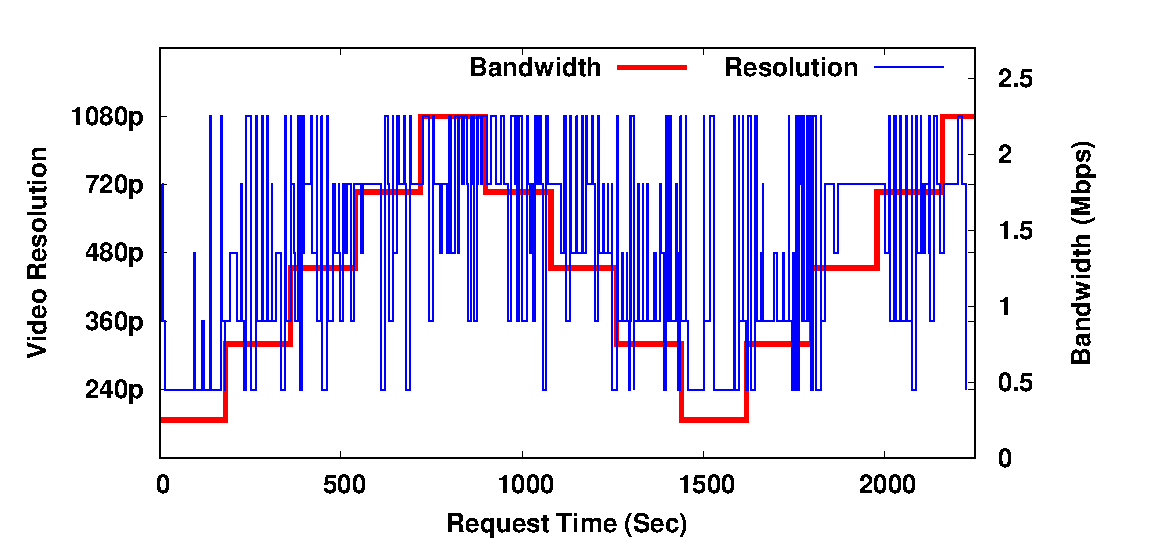
\includegraphics[scale=0.7]{img/replay/resolutionchange}
	\caption{\acs{DASH-IF}: Video resolution adaptation}
	\label{fig:reply-reso}
\end{figure}

\begin{figure}[!t]
	\centering
	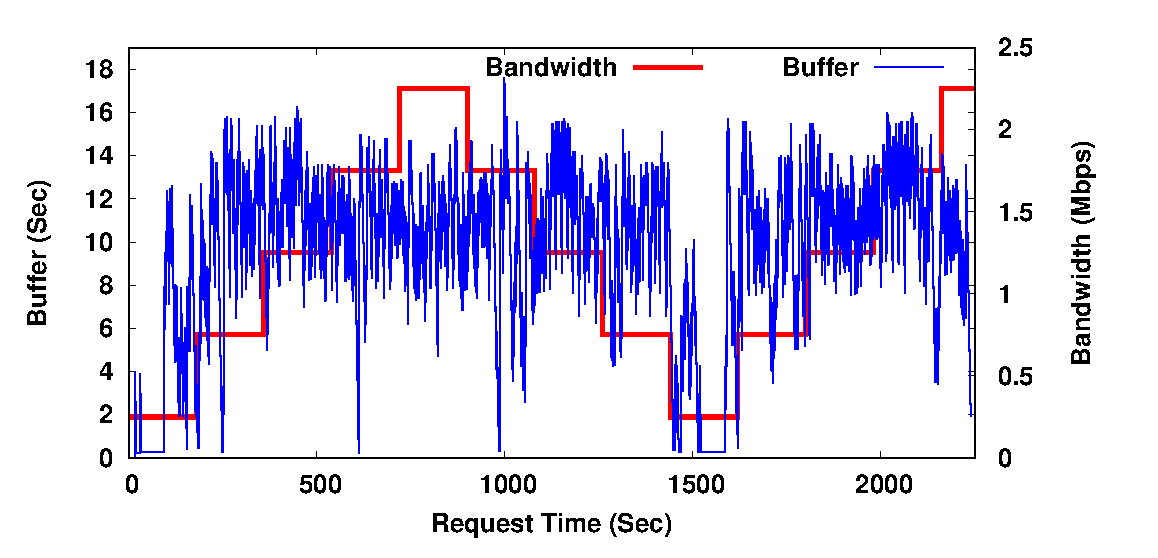
\includegraphics[scale=0.7]{img/replay/bufferchange}
	\caption{\acs{DASH-IF}: Receive buffer evolution}
	\label{fig:buf_reply}
\end{figure}

\begin{figure}[!t]
	\centering
	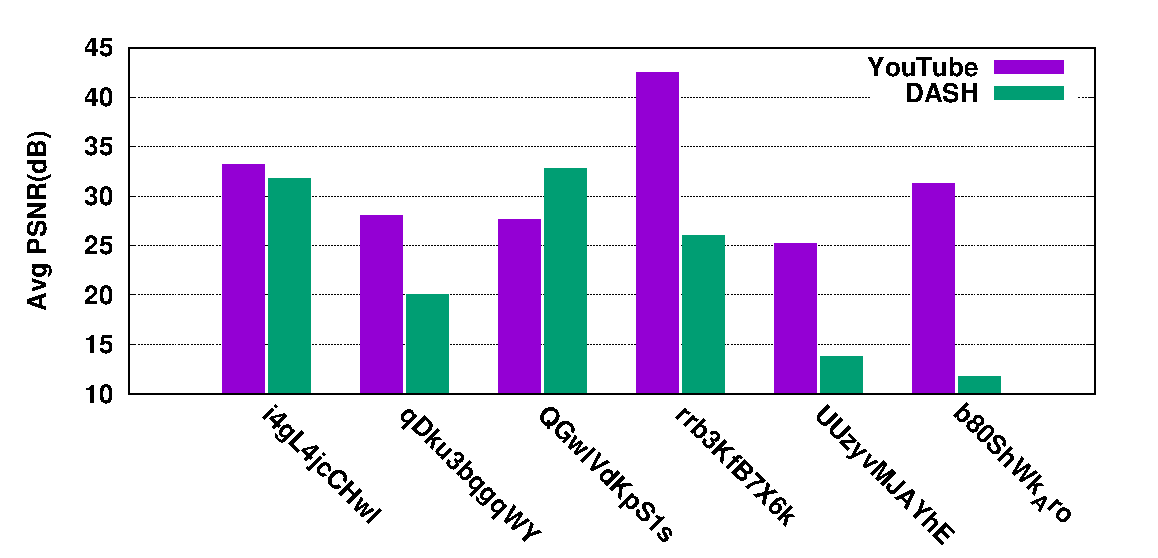
\includegraphics[scale=0.7]{img/plot_qoe}
	\caption{\acs{PSNR} comparison}
	\label{fig:qoe_ytds}
\end{figure}


\fig\ref{fig:reply-reso} shows the video resolution adaptation for a sample video with respect to time. We see significantly more number of fluctuations in video resolutions, compared to what we observe in YouTube through the evolution of values associated with the $itag$ parameter. Therefore, the $itag$ parameter provides a reference for comparison between YouTube and another \ac{DASH} based protocol implementation, in terms of the video quality adaptation over multiple available resolutions. Further, the $rbuf$ parameter helps us to compare the performance between YouTube and another \ac{DASH} based protocol, in terms of receive buffer occupancy. \fig\ref{fig:buf_reply} plots the receive buffer evolution of \ac{DASH-IF}. By comparing this figure with \fig\ref{fig:chap03s1:rbuf_evol}, we can see that YouTube buffer evolution is more consistent as compared to \ac{DASH-IF} buffer evolution, the obvious reason being that \ac{DASH-IF} does not use a sophisticated buffer management policy as YouTube does, where the segment lengths of the incoming video chunks are adapted based on the status of the receive buffer.
%\noteng{Not sure whether it is obvious from the result - needs more explanantion}

%
% \begin{figure}[h]
% \centering
% 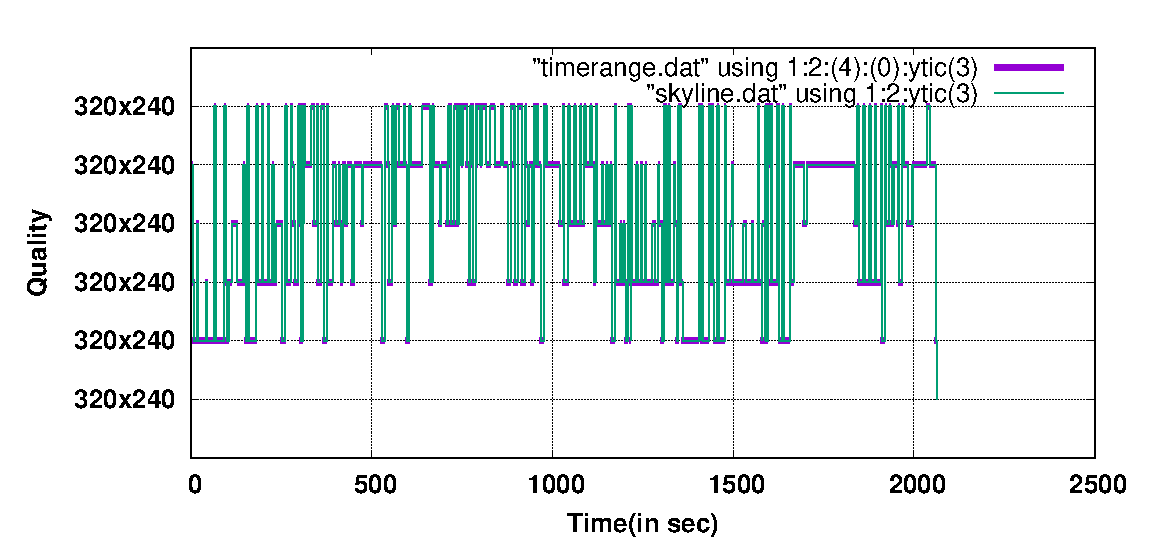
\includegraphics[width=2.5in]{img/replay/plot_timerange}
% \caption{Plot for time range of different quality in open dashjs with same configuration}
% \label{fig:timespent_replay}
% \end{figure}
%
\subsection{Comparison in Terms of QoE: Use of $itag$ Parameter}

It can be noted that comparing the \ac{QoE} of YouTube with that of another \ac{DASH} implementation is not straight-forward. By observing $itag$ values, we can say what particular video quality is requested by YouTube client at a given time, although the actual perception will depend on the resolution at which the user renders the video. For example, a $240p$ video may give good user perception if it is played on a smart-phone screen, although the quality of that video rendering will be bad over a high resolution desktop. Therefore, we use the following methodology for finding out the \ac{QoE} of a YouTube video. We take a reference resolution, and convert all the video chunks to that resolution from the one specified by the $itag$ parameter. Similarly, we observe at what resolution the video gets rendered in \ac{DASH-IF} player and convert that resolution to the reference resolution. Now both YouTube rendered video and \ac{DASH-IF} rendered video are in same resolution, and we can compare them using the standard \ac{QoE} metric. In \fig\ref{fig:qoe_ytds} we show the comparison between YouTube and \ac{DASH-IF} in terms of \ac{PSNR}, for six reference videos. The X-axis shows the video IDs as per YouTube. In general the \ac{PSNR} is low for \ac{DASH-IF}, although it gets higher for some cases as \ac{DASH-IF} may download more number of higher resolution frames.

It is interesting to observe from our study that \ac{DASH-IF} works in a best-effort manner, whereas YouTube uses a progressive approach which is similar to the elastic behavior of \ac{TCP} traffic. Just like \ac{TCP} increases the data rate until it experience congestion, YouTube goes for higher quality video and higher streaming rate till the receive buffer is steady. \ac{TCP} drops data rate in a conservative approach as it experience congestion, and similarly YouTube drops video quality and segment length when it observes declined buffer size.


\section{A Predictive Model for Data Consumption During ABR Streaming}
\label{chap03s1:sec:model}

As mentioned in \S\ref{chap03s1:sec:introduction}, we realize that early prediction of data consumption even before a video has actually played, can be extremely useful while streaming videos in a challenging scenario.
In order to achieve this, we propose an analytical model, with a machine learning based classifier, which we describe next.

Let $i,\ 1 \leq i \leq n$ represent an $itag$ value; where $n$ is the total number of $itag$ values used by YouTube.
Let $\lambda_i$ represent the frame rate for $itag$ value $i$; from our observations, frame rate per $itag$ is constant.
Let us also consider an indicator variable $p(t)$, where $p(t)=1$ denotes that at a particular instance of time ($t$), a key-frame has arrived.
Let $\alpha_i$ be the size of a key-frame (in bits) for $itag$ value $i$, and $\beta_i$ be the size of an intra-frame (in bits) at $itag$ value $i$.
Therefore, the amount of data arrived (in bits) in a single frame for $itag$ $i$, say $\mu_{i}$, is given by:
\begin{equation}
 \mu_i = \lbrack p(t).\alpha_i + \left\{1-p(t)\right\}.\beta_i \rbrack
\end{equation}
Since frame rate is $\lambda_i$, the amount of data (in bits) downloaded per unit time for $itag$ $i$, is given by:
\begin{equation}
 \delta_i = \mu_i.\lambda_i
\end{equation}
Let us consider an infinitesinally small time instance $dt$, during the YouTube streaming process. The amount of data downloaded per instance of time would be: $\delta_i.dt$, for a single $itag$ $i$.
However, data may be downloaded for different $itag$ values at the same time instance, which is where the data wastage stems from.
Let us define another indicator variable $q_{i}(t)$, where $q_{i}(t)=1$ indicates that data corresponding to $itag$ $i$ has been downloaded at time $t$.
In such a scenario, the total amount of data (in bits) downloaded in playback time duration $\tau$, is given by:
\begin{equation}
 \Delta = \int_{0}^{\tau} \left\{\sum_{i=1}^{n} q_{i}(t).\delta_{i}\right\}\ dt %= \int_{0}^{\tau} \lbrack \sum_{i=1}^{n} q_{i}(t)\lbrack p(t).\alpha_i + \left\{1-p(t)\right\}.\beta_i \rbrack.\lambda_i\ dt
\end{equation}
$\Delta$ is the measure of {\it data consumption} due to YouTube playback.\\
Let us also define $f(t)$, which is the maximum $itag$ value at time $t$, for which data is available (since data may be available for multiple $itag$ values simultaneously):
\begin{equation}
 f(t) = max\{i\}\ \forall i\ :\ q_{i}(t) = 1
\end{equation}
Therefore, the data (in bits) actually played by the YouTube player in time $\tau$, is given by:
\begin{equation}
 \rho = \int_{0}^{\tau} q_{f}(t).\delta_{f}\ dt
\end{equation}
$\rho$ is therefore the measure of {\it productive data} downloaded during YouTube streaming.
Consequently, data wastage ratio (say $\omega$), is defined as:
\begin{equation}
 \omega = \frac{\Delta - \rho}{\rho}
\end{equation}
The key to determining $\Delta$, $\rho$, and thereby $\omega$, is to estimate the values of $q_{i}$ for all $i$, at every time instance $t$.

\subsection{Classification Problem} For every $itag$ value $i$, we consider $\frac{1}{\lambda_i}$ (inverse of frame rate) as the sampling interval, since $1$ frame arrives every such interval.
We hypothesize that the value of $q_i(\hat{t})$ (where $\hat{t}$ indicates a sampled time instance) depends on the following factors -- (1) $\beta(\hat{t}-1)$ (bandwidth at previous instance), (2) $\beta(\hat{t})$ (bandwidth at current instance), (3) $i(\hat{t}-1)$ ($itag$ at previous instance), and (4) $p(\hat{t})$ (presence of key-frame at current instance).
We identify that estimating $q_i(\hat{t})$ is a binary classification problem, with every $q_i(\hat{t})$ assuming a value of either $0$ (absence) or $1$ (presence) of data of $itag$ $i$ at time instance $\hat{t}$.

\subsection{Model Accuracy} A machine learning based classifier is employed for this purpose -- we use Weka~\cite{witten2016data}, a machine learning tool, and select the Random Forest classification~\cite{breiman2001random} technique, with $100$ iterations ($I=100$) and unlimited depth ($K=0$) as hyperparameters.
In the classification technique, we try to predict the value of $q_i(\hat{t})$ using the four parameters mentioned above as classification features.
The results (\emph{\textbf{average precision = $0.86$, average recall = $0.85$, and average accuracy = $85.75\%$}}) across all $itag$s indicate high classification prowess, which validates our hypothesis regarding parameters affecting $q_i(\hat{t})$.
Using this model, a user can predict the amount of data consumption for YouTube video streaming.
